\documentclass[12pt]{article}

\usepackage{a4wide}
\usepackage{graphicx}
\usepackage{paralist}
\usepackage{hyperref}
\usepackage{parskip}

\setlength{\skip\footins}{2em}
\interfootnotelinepenalty=10000

\title{Project Information Security: \\ \textbf{Securing an Online Exam}}
\author{Pieter De Baets, Gilles Jacobs,\\ Jasper Van der Jeugt, Toon Willems}

\begin{document}

\maketitle
\newpage
\tableofcontents

\newpage

\section{Introduction}
\label{sec:introduction}

Designing an exam system is a subject that we, as students, can highly relate
to. Exams are an essential part of our education system and each of us has
pondered the design of an ideal exam system before as it's the target of our
daily activities.

Sadly the contents of exams and interrogation techniques are not part of this
assignment, as we might have some good ideas for that as well. Instead we will
only discuss the technical and practical organisation of exams, and more
specifically, exams that are taken over the public internet.

In this report, we discuss the challenges and attack vectors that are inherent
with such a setup, and provide practical solutions.

\section{Requirements and Architecture}
\label{sec:requirements}

We chose to design a system with a central component, i.e., a server, to which
the different clients can connect. For users, it would appear that this central
server is their exam platform. This is not true however, as responsibilities and
software is distributed over all platform participants.

One disadvantage of this approach is that this server needs to be trusted to
some extent by the users, which we tried to limit as much as possible.

\subsection{Assumptions}
\label{subsec:req-assumptions}

We need to assume that every user (students as well as professors) are
registered on this platform. These accounts can be created when a student
enrolls in the institute, or when a professor is employed.

The users of the platform should be able to verify that they are indeed talking
to the official platform instance, and not to some attacker posing as the
platform. This problem is mostly alleviated by using HTTPS with a trusted
certificate for all communication. Next to this, the server also uses a key pair
for signing messages it generates. We assume that its public key is known to the
users so it can be used for verification.

We use asymmetric encryption mechanisms for many features, so we also need to
assume that each user has a key pair assigned. These key pairs can be created at
the same time as the accounts, with some option to reset a key pair when it has
been compromised. The platform only requires a user's public key, the private
key is to be kept secret by the user.

Ideally these keys are also signed by an official entity so that users can
lookup and trust public keys found using a public key infrastructure.

\subsection{Functionality}
\label{subsec:req-functionality}

\subsubsection{Logging in}
\label{subsubsec:req-func-auth}

Users (students and professors) should be able to log in to the application,
prove their identity and receive the correct permissions. This means we need
some kind of authentication: it is obvious that a student should not be able to
pose as a professor and modify an exam, or submit answers for another student.

\subsubsection{Setup and distribution of exams}
\label{subsubsec:req-func-exams}

The professor needs to be able to distribute an exam to the students. He first
uploads it to the central server, and selects a number of students. These
students can download it from the server at some point in time, also specified
by the professor.

Integrity and non-repudiation are important here: we must ensure the students
see the same exam that the professor posted, without any alterations, and that
they are able to verify that the exam was authored by the professor.
Furthermore, only the selected students should be able to see the exam, and we
have to make sure they cannot view the exam before they are allowed to.

Another goal of the exam platform is to simplify the disclosure of the exam
questions for the professor. We provide 2 solutions for this:

\begin{enumerate}

\item \textbf{Timed exam release}: when setting up the exam, the professor can
choose the period of time during which the exam should be available to selected
students. Outside this time period the system will not allow any access to the
data.

\item \textbf{Locked exams}: as storing the exam unencrypted on the server is a
potential, albeit small, risk (see \autoref{subsec:req-attacks}), we provide the
professor with the additional option of uploading an encrypted version of the
exam, which the system can unlock later when a passphrase is given.

This is a minor action that can be done a couple of hours in advance of the
exam, and which provides an extra layer of security around the exam data.

\end{enumerate}

Finally, when students download the exam, they need to receive some form of
proof of their interaction with the server as part of the audit trail. This
might not be very important in this phase of the exam procedure but it will be
in the next section.

\subsubsection{Receiving answers from students}
\label{subsubsec:req-func-answers}

% To discuss:
% * should be impossible to alter answers
% * only professor can read them
% * student needs proof of submission by server

After completion of an exam, the student needs to return his answers to the
professor. He does this by uploading them to the central server. We have to
ensure that these answers can not be altered on the server (or that
modifications will be detected) and that they cannot be repudiated. These
answers are also confidential and should only be readable to the professor.

As a confirmation of his answer submission, the student receives a proof of
submission from the server. With this receipt, he can prove that he submitted
the given answer file at the current time to the server, in case of a server
error or any dispute.

\subsubsection{Distributing exam results}
\label{subsubsec:req-func-results}

% To discuss:
% * only student can see his result
% * student should be able to verify that professor authored results

When the professor has corrected a student's answers, he can upload the
corresponding exam results to the server for the student to see.

It is important that these results can only be viewed by the student they are
intended for. They should also be immutable and verifiable authored by the
professor.

\section{Concrete implementation}
\label{sec:implementation}

% Some implementation details, mention the actually used algorithms here.

We built a proof-of-concept application using Ruby on
Rails\footnote{\url{http://rubyonrails.org/}} incorporating the main
functionality. All communication with this web application will occur over HTTPS,
as noted earlier.

A number of operations in the application rely heavily on locally available
keys, which we did not want to store on the server for security reasons.
Therefore we also wrote some small shell scripts which the user can execute on
his local machine to perform the required encryption and signing operations,
using OpenSSL and GnuPG.

An advantage of scripting the use of these standard security packages is that
the used security is very transparent. A paranoid user that does not trust the
central server can easily read these scripts and perform the required steps
himself.

We will now discuss some more implementation details for each subsystem.

\subsection{Authentication}
\label{subsec:impl-authentication}

\begin{figure}[ht]
  \begin{center}
  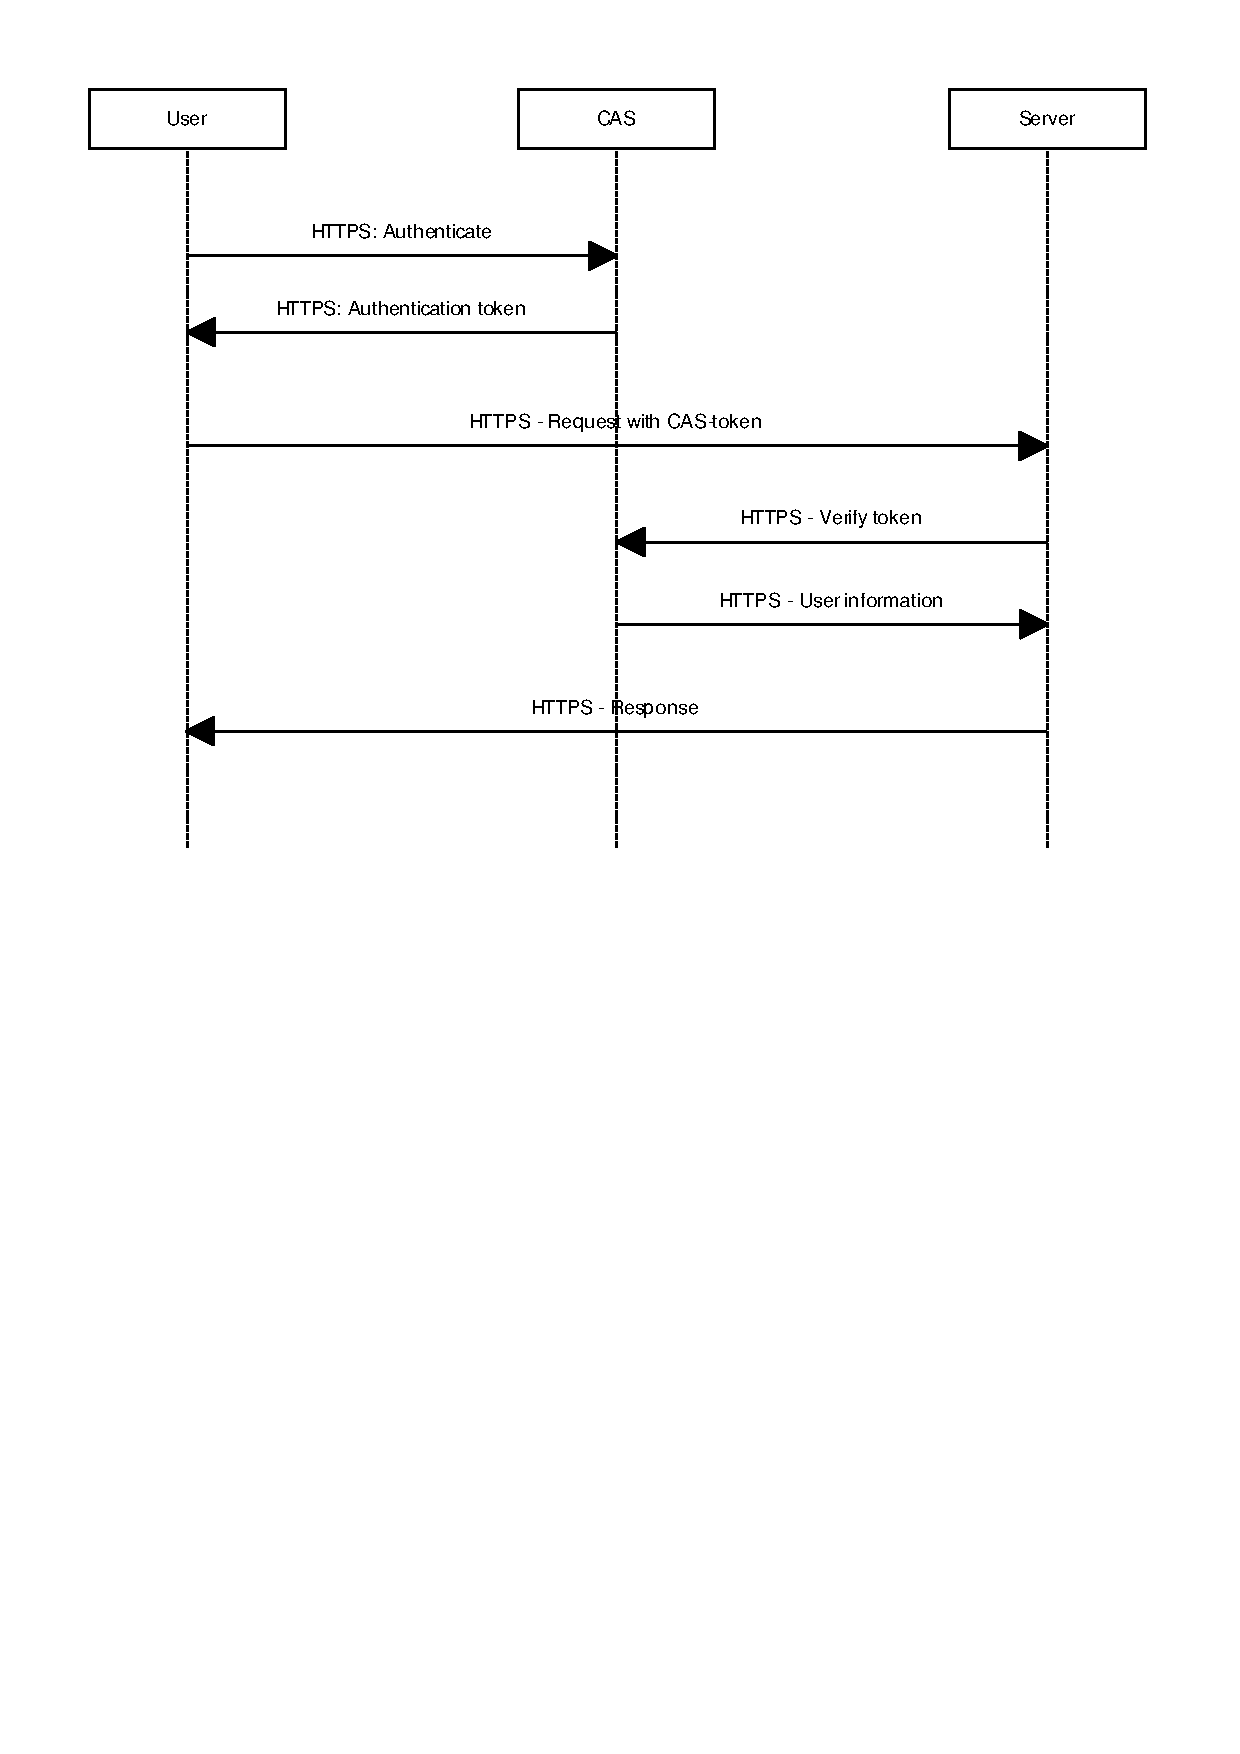
\includegraphics[width=0.9\textwidth]{images/login.pdf}
  \caption{Messages exchanged when logging in}
  \label{fig:login}
  \end{center}
\end{figure}

It is definitely possible to design a custom secure authentication solution.
However, given the setting, we chose for a more realistic option. Most large
organisations already have an in-house authentication gateway which applications
can use. This way authentication can be organised securely across the whole
organisation without much effort to application developers.

For our proof-of-concept we integrated with Ghent University's Central
Authentication
Server\footnote{\url{http://helpdesk.ugent.be/webhosting/en/cas.php}} (CAS)
which is an implementation of the publicly available CAS
protocol\footnote{\url{http://www.jasig.org/cas/protocol/}}. The basic exchange
of messages between user, CAS server and application server can be seen in
figure~\ref{fig:login} and is detailed below.

\begin{enumerate}

\item The user has no active session on the exam server and is redirected to the
authentication server (referencing the exam server as source of the
authentication request).

\item The authentication server verifies the identify of the user. In Ghent
University's case, this is a basic password authentication scheme (in which
hopefully a secure hash of the password is used instead of a plaintext version),
but more advanced options (e.g.\ smart cards, biometrics, \dots) are possible as
well.

\item When authentication has succeeded the authentication server generates a
security token and returns the user to the exam server, carrying this token.

\item The exam server will then contact the authentication server and confirm
the user's identity using this token. The use of the token is strictly regulated
to prevent abuse: only the requesting service can use it, it is only valid
during a small time frame and can be used only once.

\item Having received this information, the exam server can now start a local
application session for the authenticated user.

\end{enumerate}

\subsection{Exam distribution}
\label{subsec:impl-exams}

%\begin{figure}[h]
%  \begin{center}
%  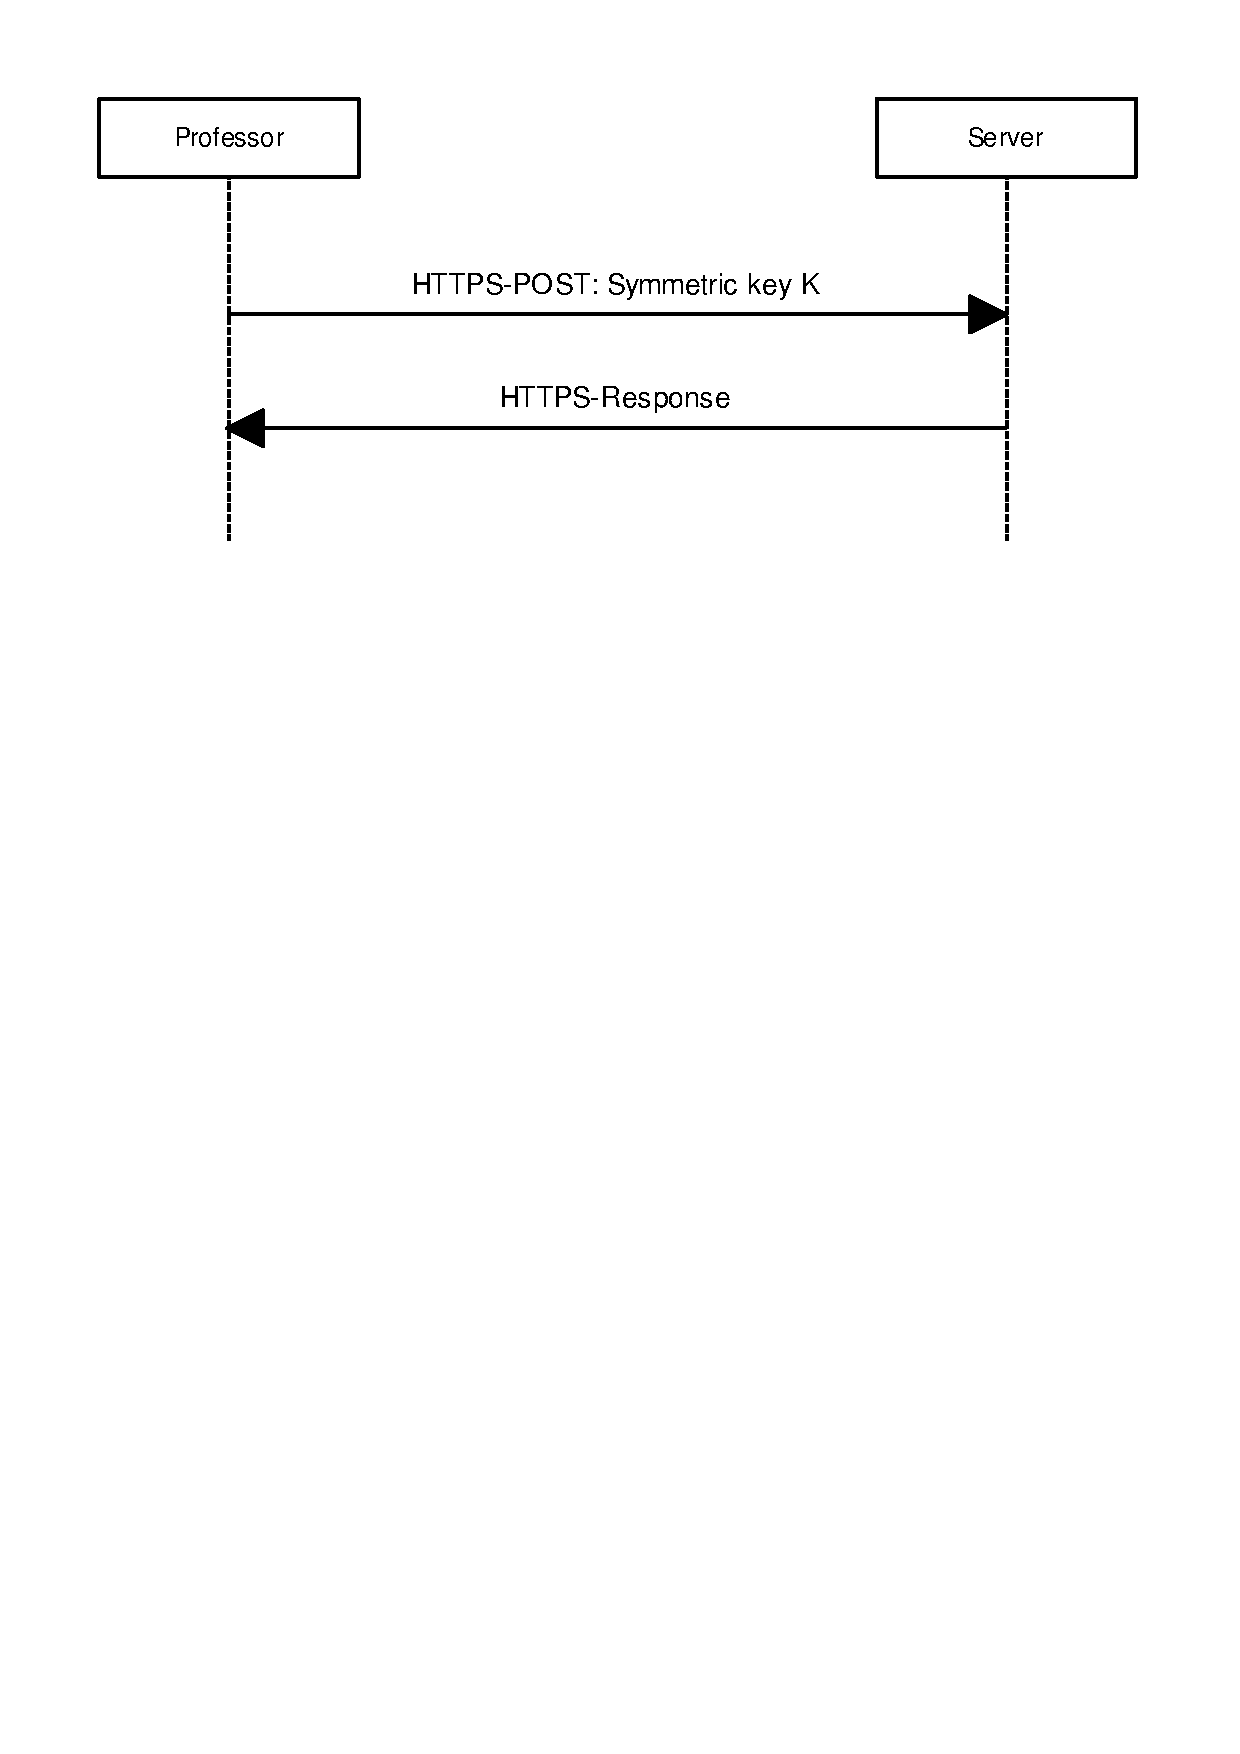
\includegraphics[width=0.6\textwidth]{images/unlock_exam.pdf}
%  \caption{Messages exchanged when unlocking an exam}
%  \label{fig:unlock-exam}
%  \end{center}
%\end{figure}

%\begin{figure}[h]
%  \begin{center}
%  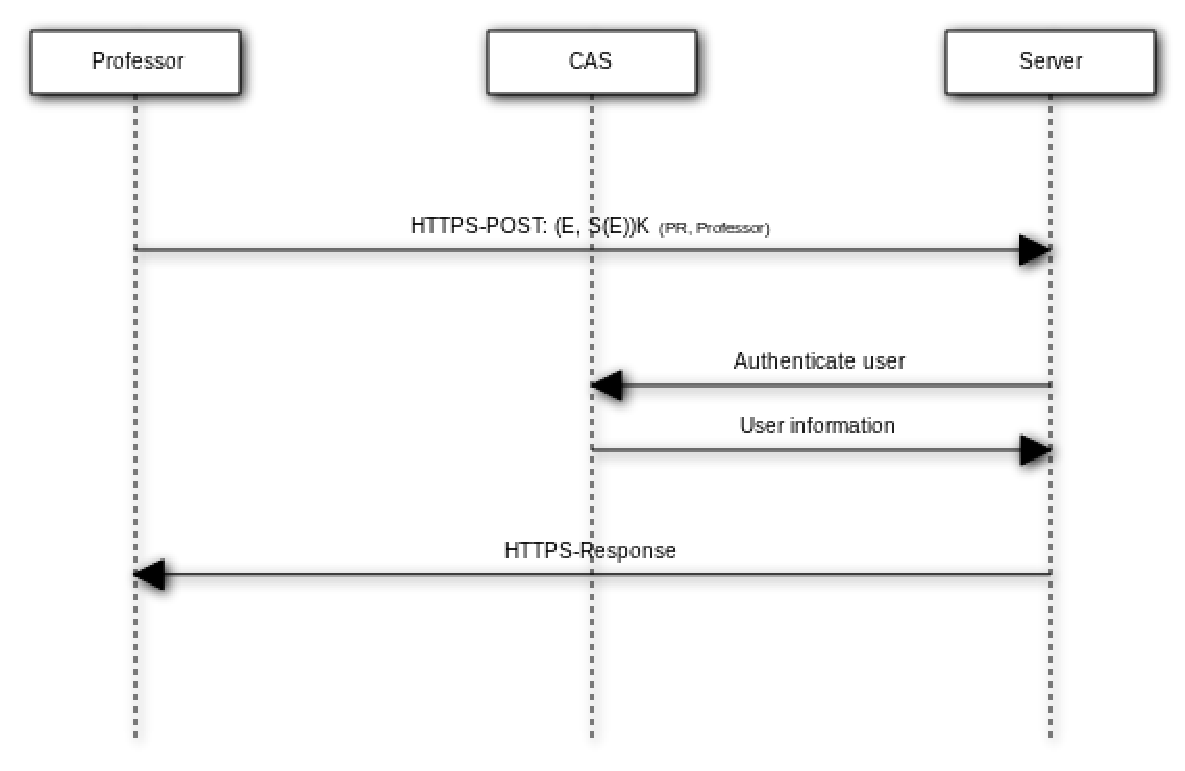
\includegraphics[width=0.6\textwidth]{images/upload_exam.pdf}
%  \caption{Messages exchanged when uploading a locked exam}
%  \label{fig:upload-exam}
%  \end{center}
%\end{figure}

%\begin{figure}[h]
%  \begin{center}
%  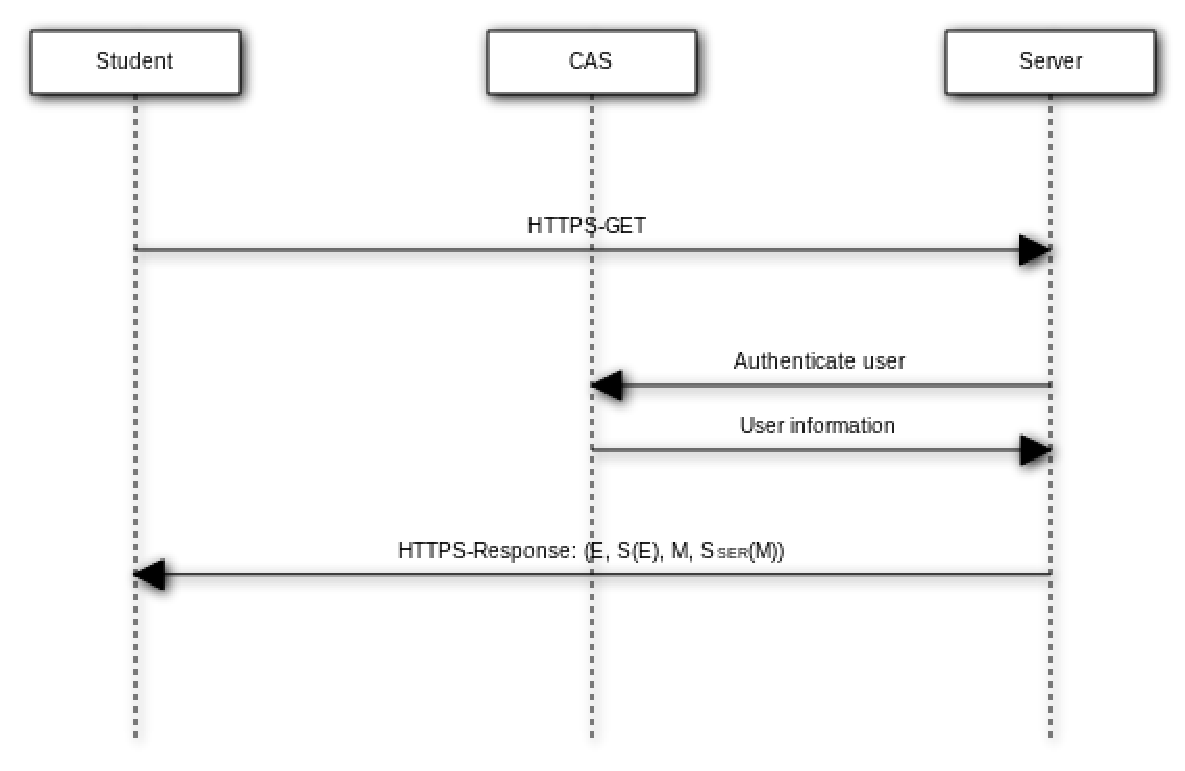
\includegraphics[width=0.6\textwidth]{images/download_exam.pdf}
%  \caption{Messages exchanged when downloading an exam}
%  \label{fig:download-exam}
%  \end{center}
%\end{figure}

We assume that a user that wants to perform any of tasks is already authenticated
to the platform, as explained in \autoref{subsec:impl-authentication}.

To \textbf{upload an exam}, the professor first needs to create an exam bundle
by running \texttt{create-exam}. This script takes as its argument the filename
of the exam and will generate a RSA/SHA-512\footnotemark{} signature of that file
using the default GnuPG keypair.

\footnotetext{GnuPG uses a SHA-1 hash by default. NIST, however, currently
recommends using a hash function from the SHA-2 family for all new applications,
e.g. SHA-512.}

Optionally, the \texttt{create-exam} script can also encrypt the exam file (see
"Locked exams" in \autoref{subsubsec:req-func-exams}). To do so, it first
creates the signature and then encrypts the file using 256-bit AES with cipher
block chaining for which the user needs to enter an encryption password.

To \textbf{unlock an exam}, the professor submits the passphrase he used when
creating the locked copy, to the server. The server will decrypt the file using
the aforementioned AES algorithm and store the unlocked copy.

When the time has come for the exam to become available, students can
\textbf{download the exam}. In addition to the exam file, the server will also
send the associated signature and a proof of the download that has taken place.
This proof is a text file which is signed with the server's private key and
contains the student's identity, the server time, the exam and a SHA5-12 hash
of the exam file that was just downloaded.

\subsection{Receving answers from students}
\label{subsec:impl-answers}

%\begin{figure}
%  \begin{center}
%  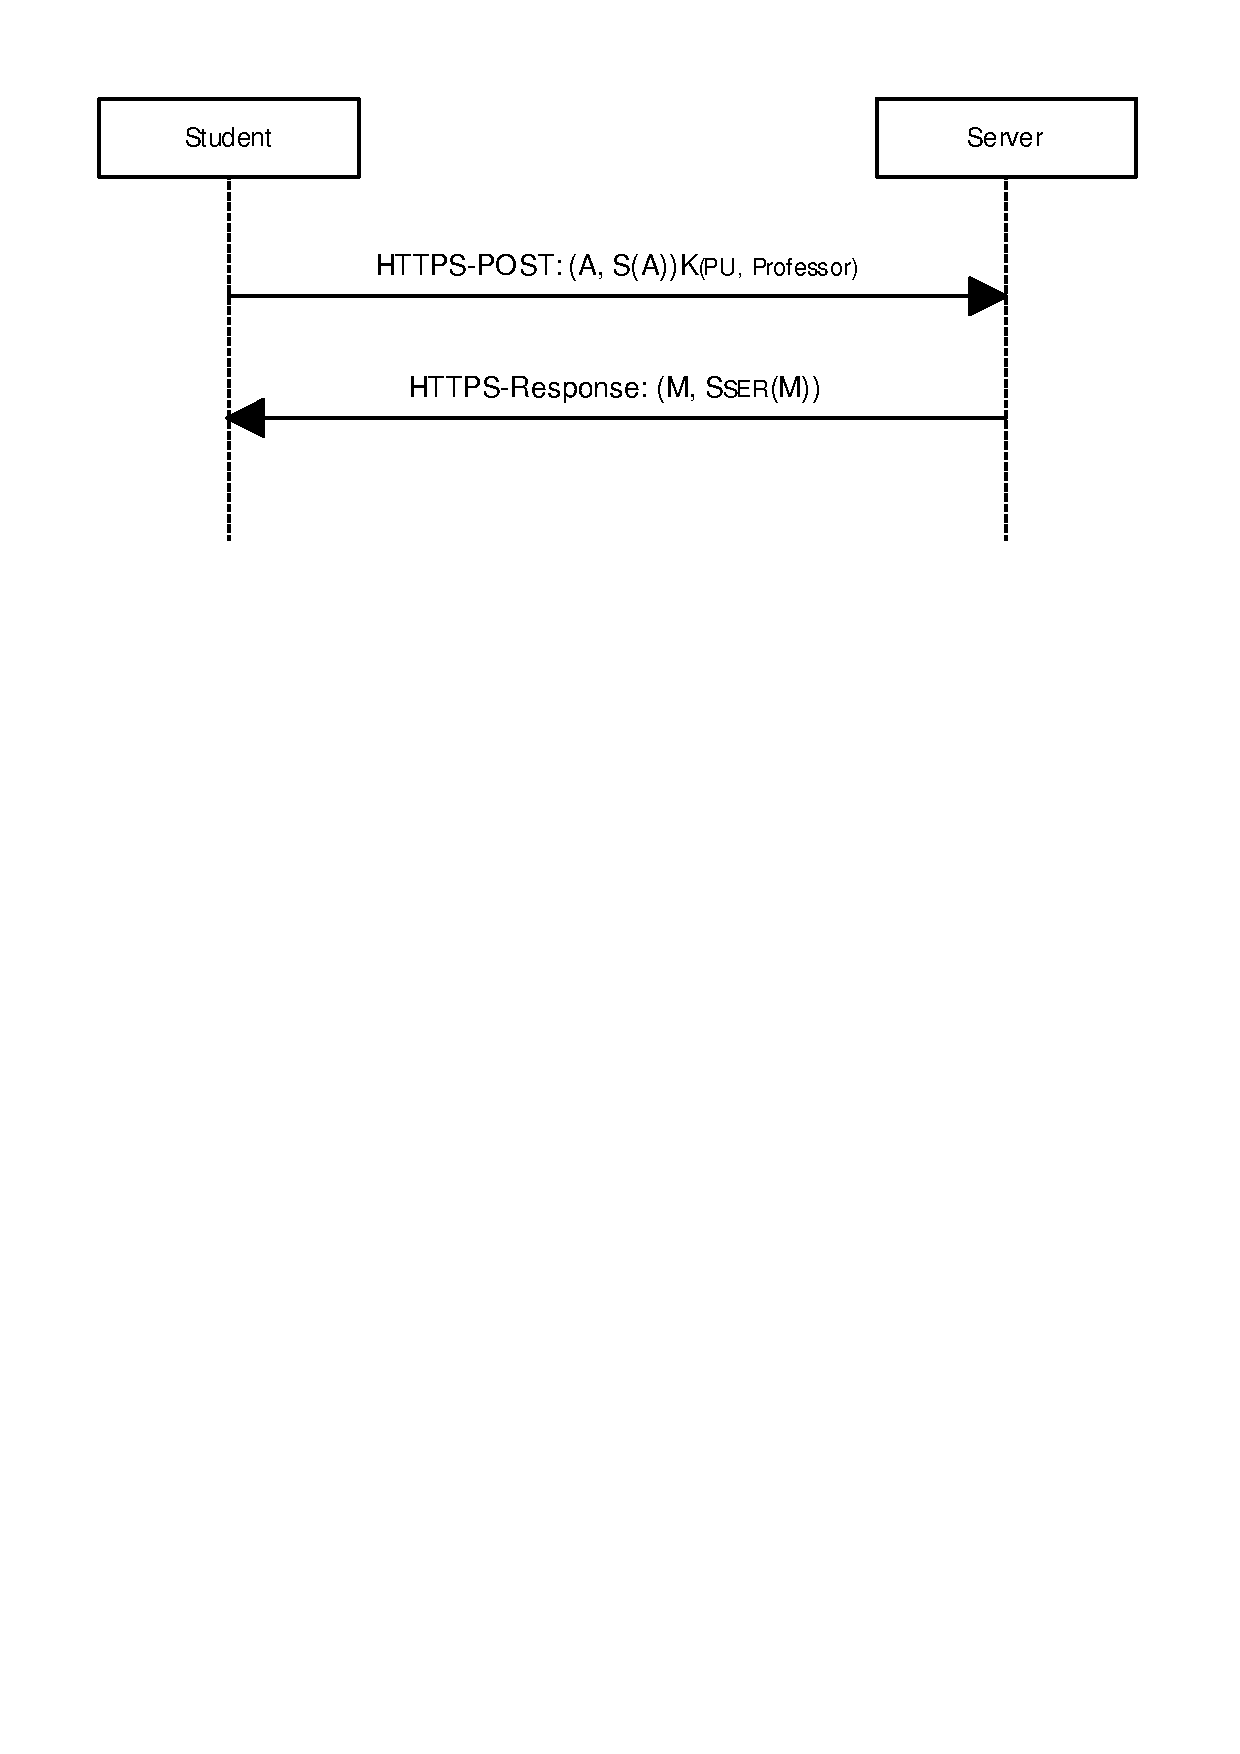
\includegraphics[width=0.75\textwidth]{images/upload_answers.pdf}
%  \caption{Messages exchanged when uploading answers}
%  \label{fig:upload-answers}
%  \end{center}
%\end{figure}

%\begin{figure}
%  \begin{center}
%  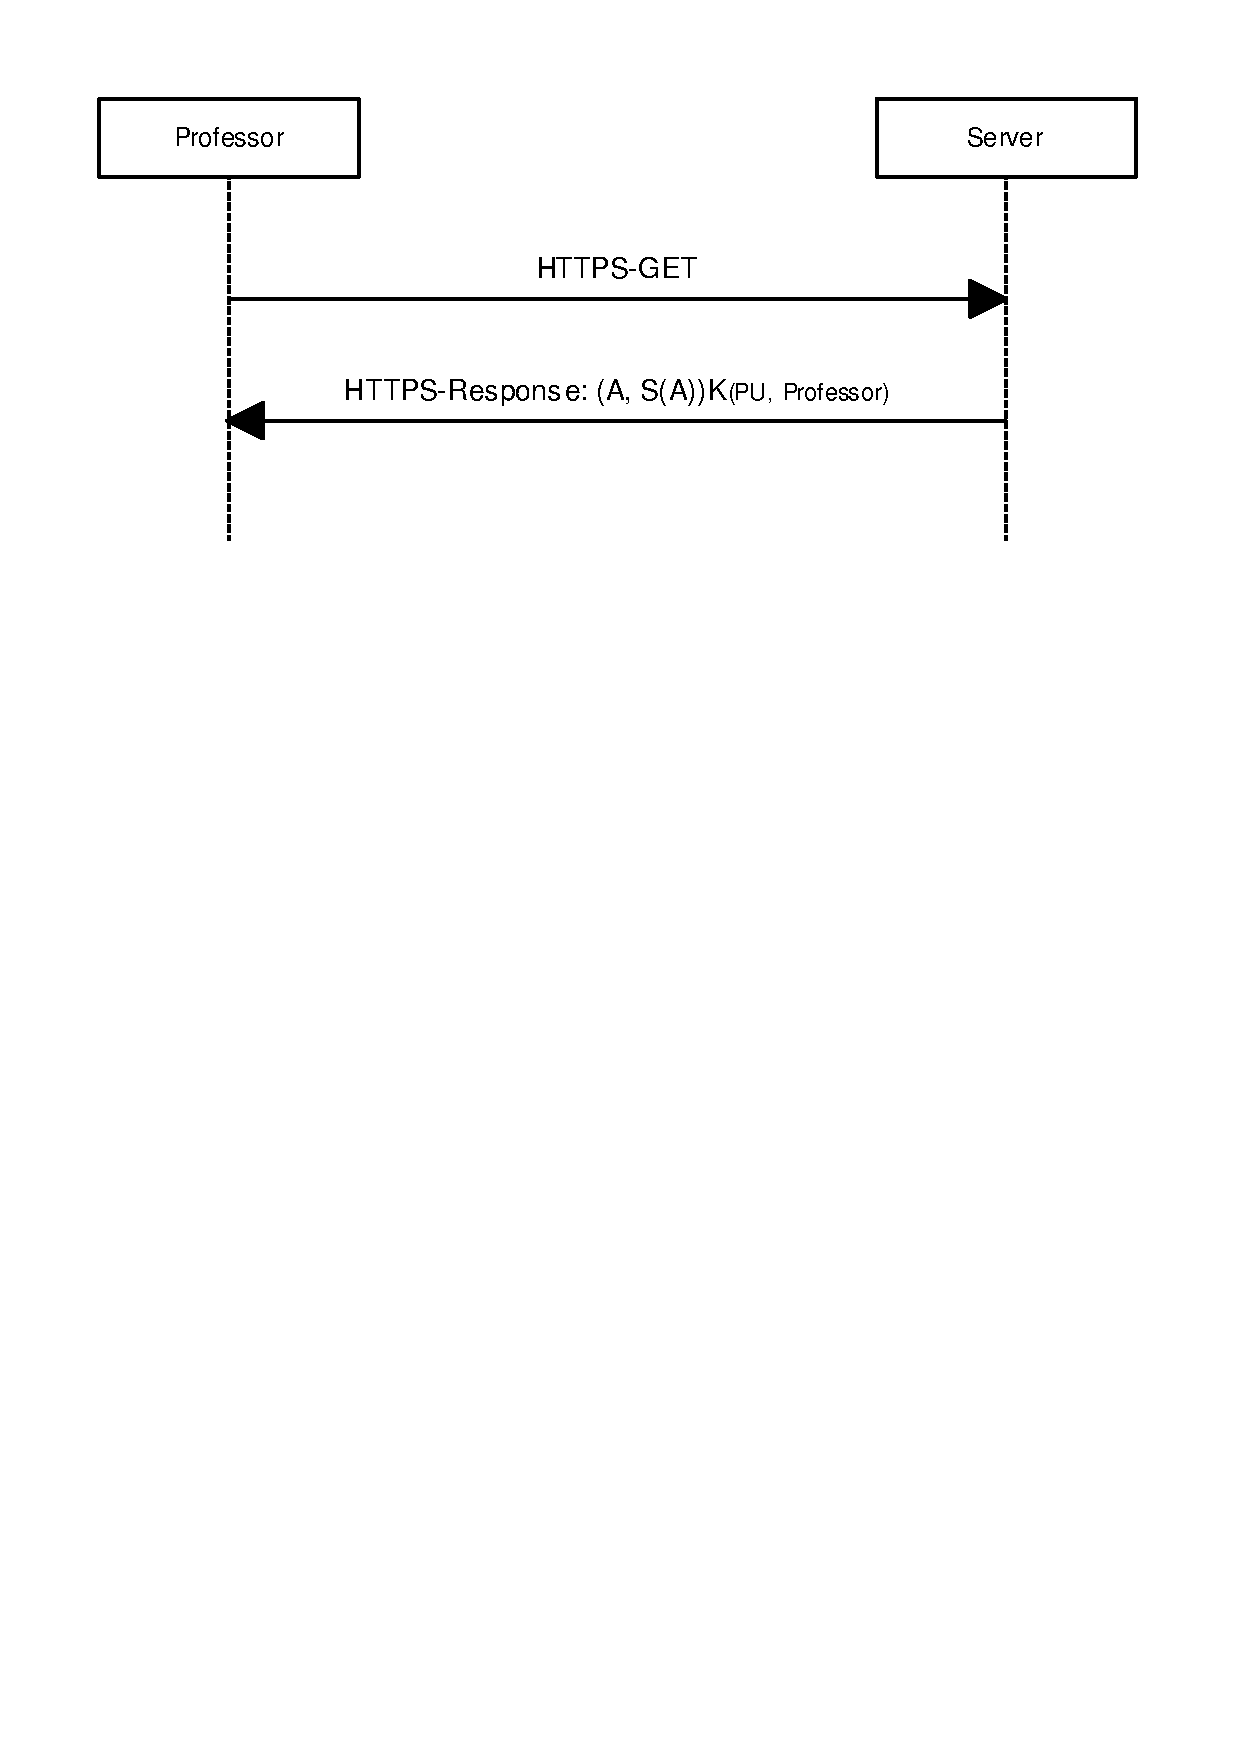
\includegraphics[width=0.75\textwidth]{images/download_answers.pdf}
%  \caption{Messages exchanged when downloading answers}
%  \label{fig:download-answers}
%  \end{center}
%\end{figure}

Again, we assume that any user of the platform is correctly authenticated before
executing one of these tasks.

To achieve the required security properties we process the student's answers with
the following process (implemented by the \texttt{create-answers} script).

\begin{enumerate}

\item To guarantee data-integrity and non-repudiation, the student will first
sign his answers with his private key. Again the RSA/SHA-512 procedure is used,
as implemented by GnuPG.

\item Another requirement is data confidentiality: only the professor should be
able to read the file. For this we use the second mode of RSA-operation:
encrypting a file for a specific person, using his public key.

We encrypt the document symmetrically (using GnuPG) with AES and a random 256
bit key. This key is then encrypted with the professor's public
key\footnotemark{} and stored with the encrypted file.

\footnotetext{Additionally we also encrypt the AES key using the student's own
public key. This way he can decrypt his answers file himself as well.}

\end{enumerate}

When receiving this encrypted package, the professor can now decrypt it using
his private key, verify the signature and finally, correct the answers given in
the file.

After submission, the student will receive a proof of submission, to complete
the audit trail. The proof is once again a text file, signed with the server's
private key.  In this case, the text file contains the student's identity, the
server time, a reference to the exam and a SHA-512 hash of the encrypted answers
file that was just submitted.

\subsection{Distributing exam results}
\label{subsec:impl-results}

To distribute the results obtained by the students, we use the same mechanism as
in \autoref{subsec:impl-answers}, but in the other direction. The mechanism is
implemented in the \texttt{create-results} script.

% The functionality of create-results would be exactly the same as
% create-answers, should we just copy them for clarity?

For each student, the professor will sign the document containing his results
with his private key (using the RSA/SHA-512 algorithm in GnuPG). This guarantees
that the results are authored by the professor and haven't been changed since.

Next, for privacy reasons, the signed package is encrypted with the student's
public key (following the same procedure as in the previous section). Now only
the student will be able to decrypt the answers.

%\begin{figure}
%  \begin{center}
%  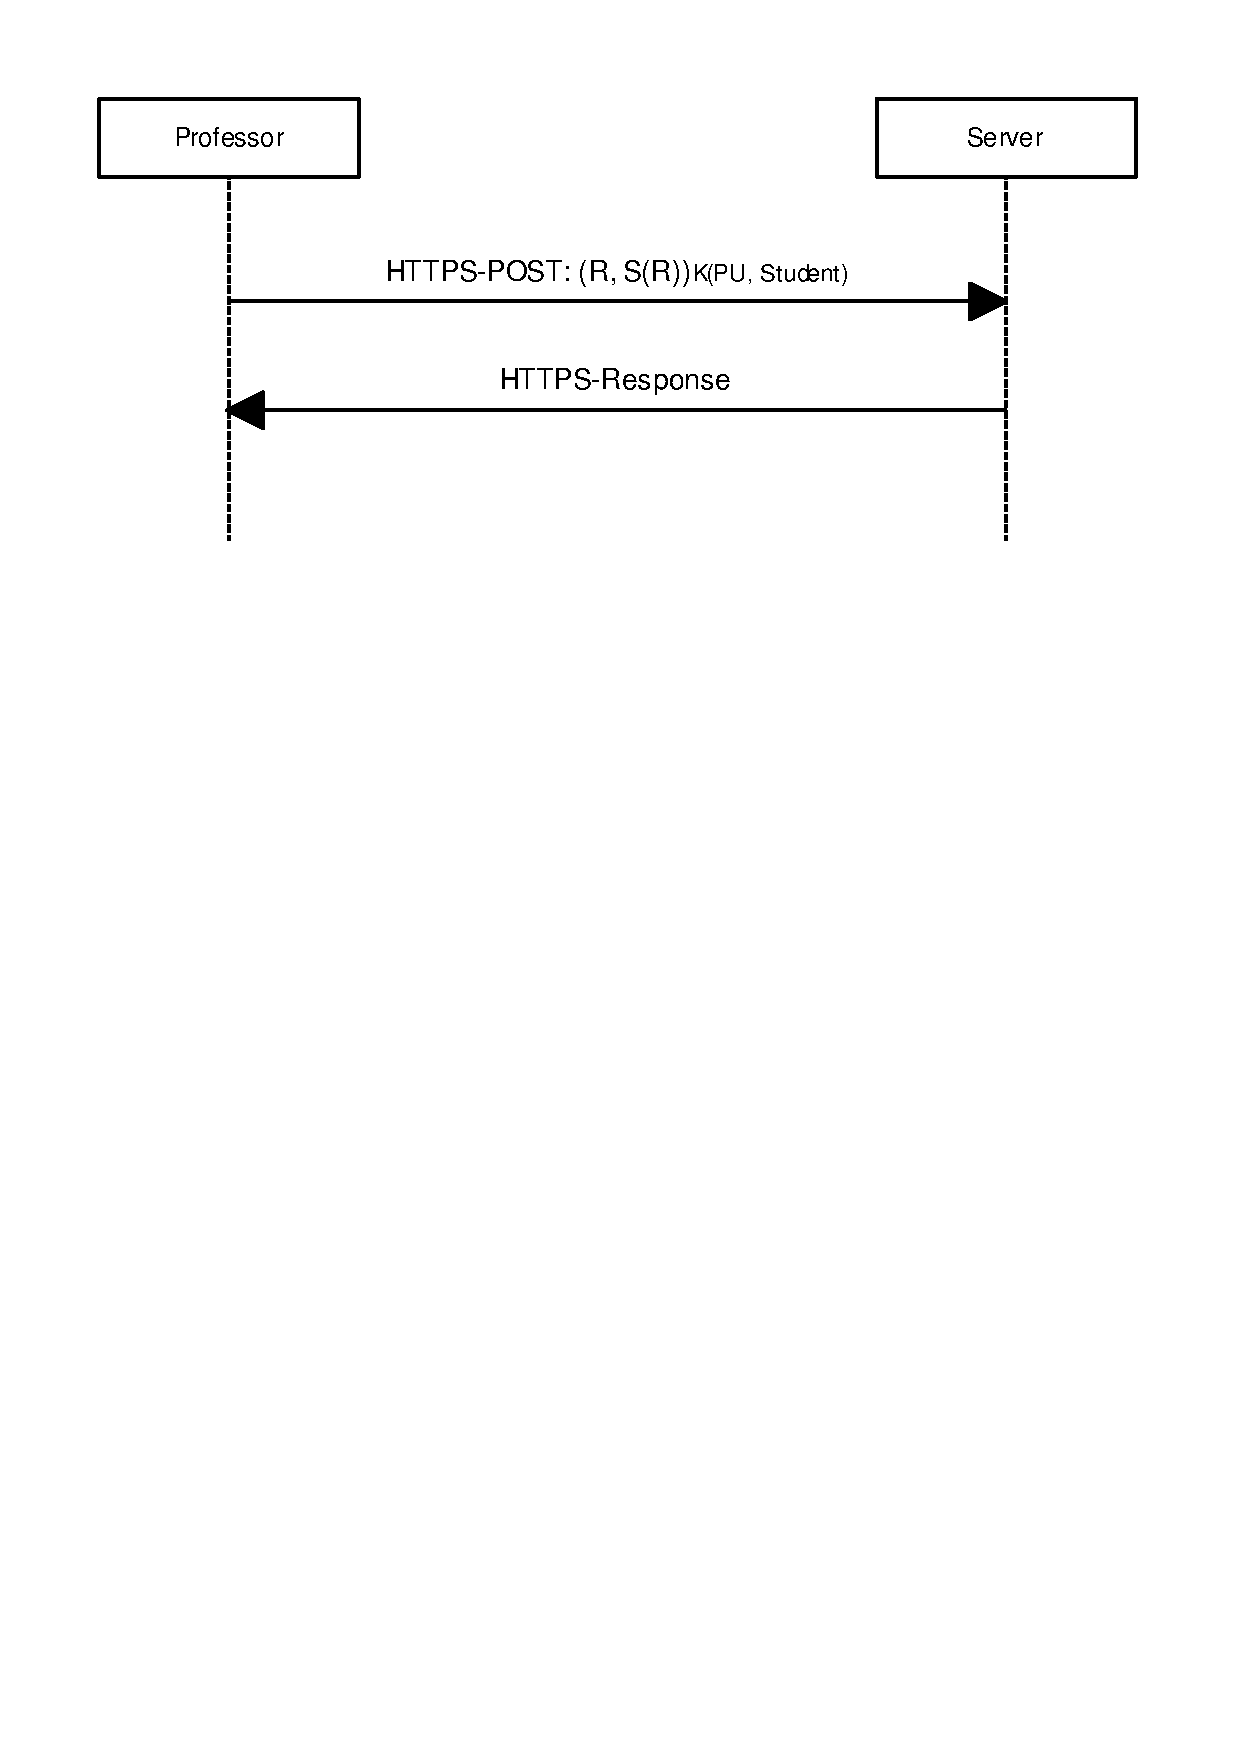
\includegraphics[width=0.75\textwidth]{images/upload_scores.pdf}
%  \caption{Messages exchanged when uploading scores}
%  \label{fig:upload-scores}
%  \end{center}
%\end{figure}

%\begin{figure}
%  \begin{center}
%  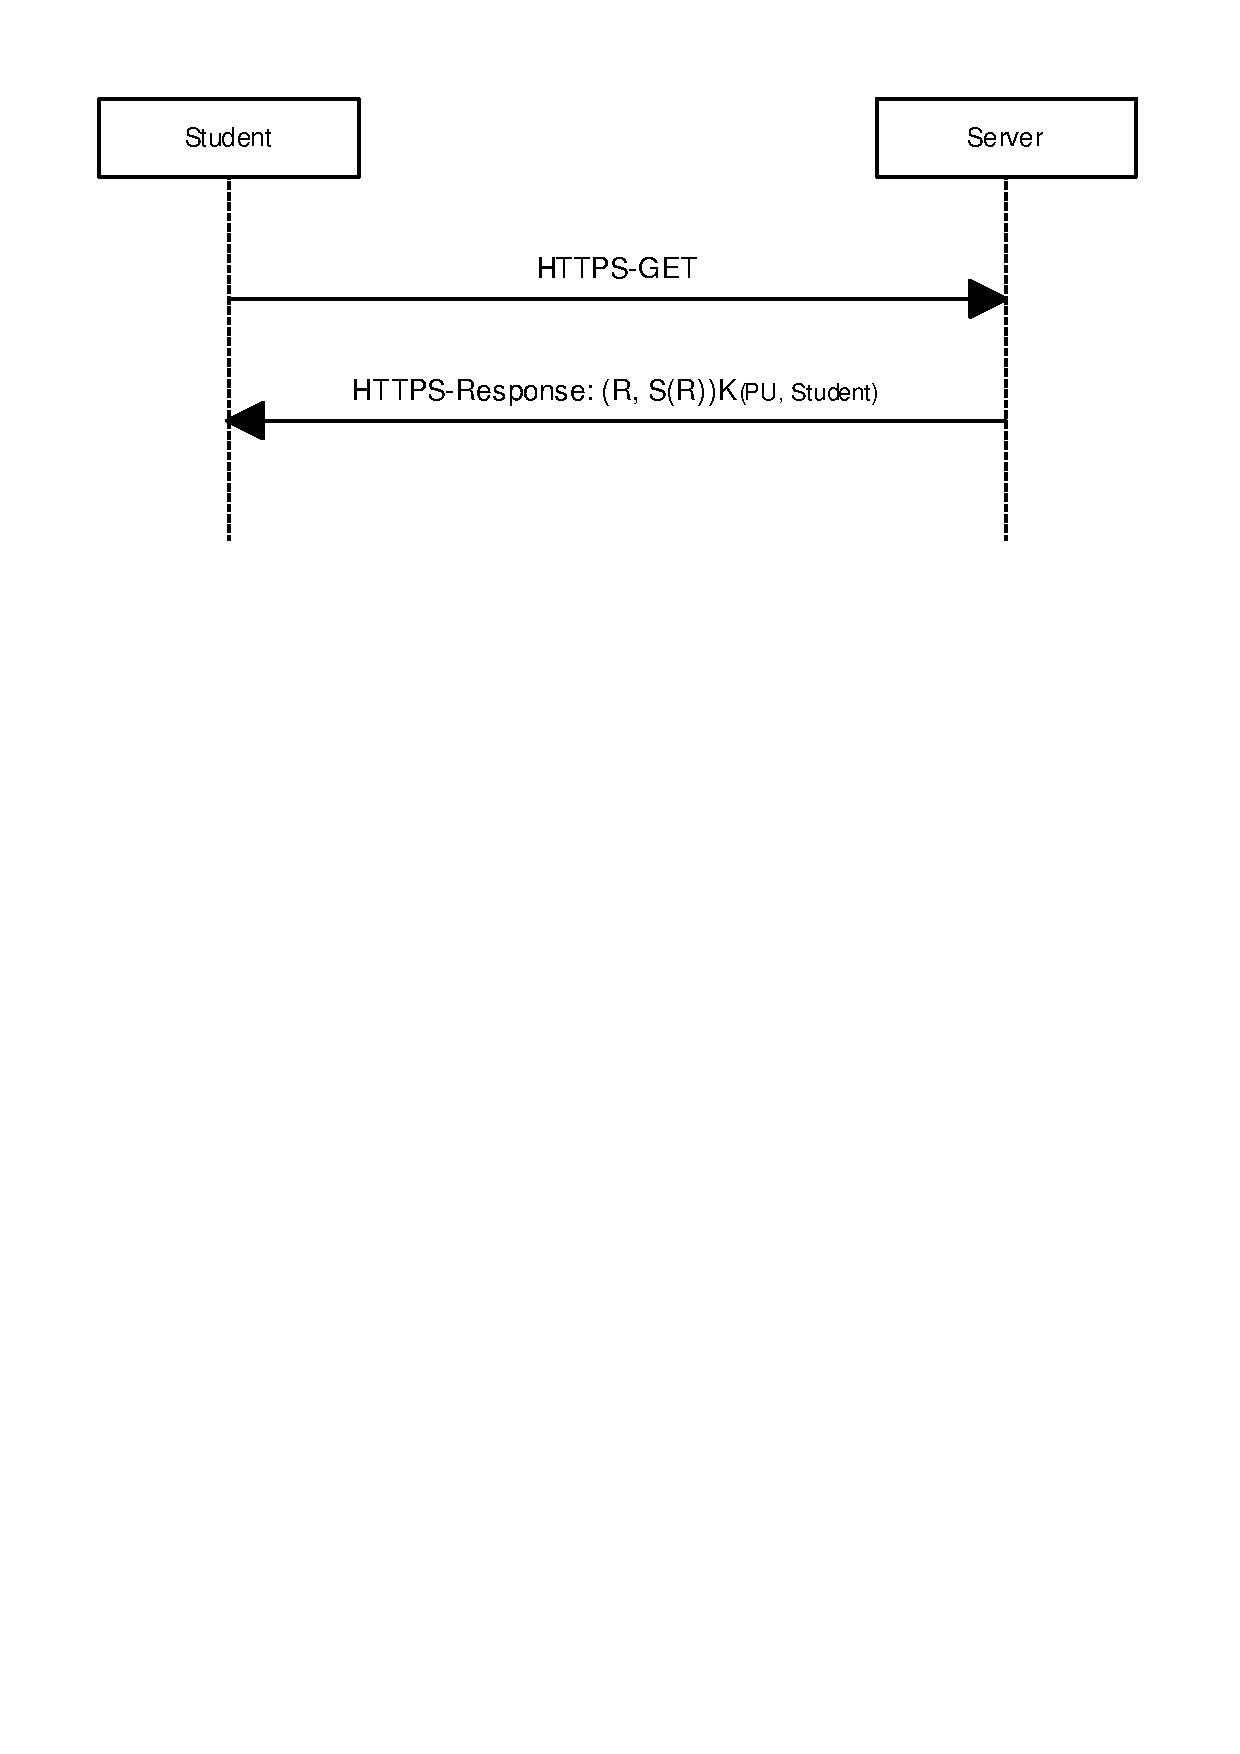
\includegraphics[width=0.75\textwidth]{images/download_scores.pdf}
%  \caption{Messages exchanged when downloading scores}
%  \label{fig:download-scores}
%  \end{center}
%\end{figure}

\section{Practical considerations}
\label{sec:practical}

In the case of perfectly trustworthy students, an online exam platform would
allow them to simply take the exam from their homes. Unfortunately, this is
often not the case, which is why all these security measures are necessary.

Even if our platform does not contain a single vulnerability, students can still
attempt to cheat in other ways. They could set up a communication channel
outside of our platform (mobile phones, passing notes) and cannot be prevented
by our application. For this reason a number of practical measures must be taken
as well.

If the students take the exam in a supervised room, we can prevent them from
using any unauthorized communication such as passing notes.

The students need access to a computer in order to use our platform. These
computers could also be used to communicate with other students using a chat
application or email. This can be prevented in two ways: a strict (whitelisted)
network setup which only allows the computer to talk to the necessary servers,
and a supervisor who keeps an eye on the computer screens---we recommend to have
both.

In such a setup, it would be advisable to use public computers instead of having
the students bringing their own laptops: this ensures that the students do not
bring more information than allowed for the exam and allows for strict control
of the software used. They do, however, need to bring their private key on a USB
stick with them. In this case, it would not be a bad idea to encrypt it with a
passphrase in case it gets stolen.

Another practical aspect is usability. Being required to run a shell script does
not form an obstruction for computer science students, but it might be a problem
for students without much technical knowledge or experience. For these students,
it would be useful to provide a friendly GUI on top of those shell scripts.

\section{Evaluation}
\subsection{Expected attacks}
\label{subsec:req-attacks}

\subsubsection{Transport layer attacks}

Several attacks are possible at this network level: sniffing traffic,
impersonating the server, a man-in-the-middle attack or a replay attack.

However, since we are using HTTPS, none of these attacks will be successful.

\subsubsection{Attacks on the server's administrative interface}

If someone were to gain access to our server, he would only be able to read the
exams when they are unencrypted. Because of our public-private key system
forgery of exams, answers and results would be impossible. The safety of our
system is not compromised if the professor chooses to encrypt the exam.

A more troubling issue is that an attacker who gains access, can possibly delete
data on to the server, without this being immediately noticeable. Our students
are protected against such dataloss however as they have the proofs of
submission that the server originally generated. Together with the original
answer bundle, a professor can then still accept their answers as a valid
submission.

Another issue is that the attacker might gain access to the private key of the
server. This would allow the attacker to generate a proof of submission
{\em after}\ he has completed his exam. This way he could gain additional time to
submit his exam. However the student needs to submit something before the
deadline of the exam. When the server receives his answers, he will immediately
send an email to the professor with the generated hash. The attacker will still
be able to update his answer file on the server and generate a correct proof of
submission, but the earlier sent hash will differ from the hash.

Some things we consider good practice for securing the server: drop all traffic
not coming from a few whitelisted locations, log all administrative actions
performed on the server for audit purposes, make regular backups (to an equally
secure server), blacklist users with abnormal traffic patterns (e.g.\ too many
failed authentication attempts).

\subsubsection{NTP attack}

To suport the timed exam release, it is critical for the server to always have a
correct time reading. Common practice is to setup a Network Time Protocol (NTP)
client on the server to regularly check and correct the clock.

If an attacker was able to gain access to the server's local network and spoof
the information from the NTP server, the exams could possibly be released
prematurely. Luckily NTP has a built-in security mechanism designed to handle
attacks like these, if configured correctly.

\subsubsection{Attacks on the website}

Because we are using a modern web framework to build this application, the most
important and common attacks against are web applications are already prevented.
The Ruby on Rails framework has built-in protection for cross-site request
forgery (CSRF) and cross-site scripting (XSS). We also use an object relational
mapper, ActiveRecord, instead of handwritten database queries, which makes it
very hard to have SQL injection attacks.

Session information is often the target of attacks on websites, as the attacker
can use that information to \emph{steal} a session. By using HTTP- and HTTPS-
only cookies to store the session information client-side we eliminate a large
number of attack vectors.

\subsection{Limitations}
\label{subsec:req-limitations}

\subsubsection{Trust}
There a number of trust issues with our system. We have to trust the honesty of
the Professor and the sysadmin. Both could abuse their power, rendering the
security of our system pointless.

\section{Conclusion}
\label{sec:conclusion}

% TODO: conclude something
During the course of this project we have designed and implemented a platform
to securely conduct exams and publish the results. This system should not only
secure the communication to and from the server, but should also ensure
confidentiality of answers and results between a student and his professor.

During the design phase, we started by securing the communication from and to
the server by using the HTTPS protocol. We then added public-private key
encryption enabling the users to verify the integrity and author of exams,
answers and results. Encryption of the answers and results also ensures
confidentiality between the student and his professor. To secure the system
against possible loss of a student's answers we created a certificate that
allows a student, if necessary, to resubmit answers without altering them.

When implementing the system we chose to use the modern Ruby on Rails
web-framework with built-in protection against common attacks on websites,
like SQL injection and cross-site scripting.

Although the presented system is secured on a technical level, it can not
prevent students from communication during an exam or using cheat sheets.
Showing how all aspects of a system influence how secure it is.


\end{document}
